
%(BEGIN_QUESTION)
% Copyright 2009, Tony R. Kuphaldt, released under the Creative Commons Attribution License (v 1.0)
% This means you may do almost anything with this work of mine, so long as you give me proper credit

Calculate the differential pressure developed by an open venturi tube measuring air speed at 80 km/h, at sea level ($\rho_{air}$ =1.21114 kg/m³, where the throat diameter is one-half that of the entrance diameter:

$$\includegraphics[width=15.5cm]{i02984x01.eps}$$

Also, how much pressure will the venturi tube develop at twice the air speed (160 km/h)?

\underbar{file i02984}
%(END_QUESTION)





%(BEGIN_ANSWER)


$\Delta P$ at 80 km/h = 4485.6 Pa 
\vskip 10pt

$\Delta P$ at 160 km/h =  17942 Pa

%(END_ANSWER)





%(BEGIN_NOTES)

%INDEX% Measurement, flow: venturi tube

%(END_NOTES)


